% Nejprve uvedeme tridu dokumentu s volbami
\documentclass[slovak,master,dept460,male,cpp,cpdeclaration]{diploma}
% Dalsi doplnujici baliky maker
\usepackage[autostyle=true,czech=quotes]{csquotes} % korektni sazba uvozovek, podpora pro balik biblatex
%\usepackage[backend=biber, style=iso-numeric, alldates=iso]{biblatex} % bibliografie
\usepackage{dcolumn} % sloupce tabulky s ciselnymi hodnotami
\usepackage{subfig} % makra pro "podobrazky" a "podtabulky"
\usepackage{verbatim}
\usepackage{cite}
\usepackage{float}
\usepackage{amsfonts}
\usepackage{url}
\bibliographystyle{unsrt}
\nocite{*}
% Zadame pozadovane vstupy pro generovani titulnich stran.
\ThesisAuthor{Michal Falát}

\CzechThesisTitle{Analýza řidiče za pomocí sférických kamer}

\EnglishThesisTitle{Driver Analysis Using Spherical Cameras}

\SubmissionDate{1. apríla 2020}

% Pokud nechceme nikomu dekovat makro zapoznamkujeme.
\Thanks{Rád by som poďakoval môjmu vedúcemu práce Ing. Radovanovi Fusekovi za pomoc a ochotu pri vypracovaní diplomovej práce}

% Zadame cestu a jmeno souboru ci nekolika souboru s digitalizovanou podobou zadani prace.
% Pokud toto makro zapoznamkujeme sazi se stranka s upozornenim.
\ThesisAssignmentImagePath{Figures/Assignment1.jpg}
% \SlovakBachelorMaleAuthorDeclaration

% Zadame soubor s digitalizovanou podobou prohlaseni autora zaverecne prace.
% Pokud toto makro zapoznamkujeme sazi se cisty text prohlaseni.ss
% \AuthorDeclarationImageFile{Figures/AuthorDeclaration.jpg}


% Zadame soubor s digitalizovanou podobou souhlasu spolupracujici prav. nebo fyz. osoby.
% Pokud toto makro zapoznamkujeme sazi se cisty text souhlasu.
% \CooperatingPersonsDeclarationImageFile{Figures/CoopPersonDeclaration.jpg}

\CzechAbstract{Hlavnou témou diplomovej práce je rozpoznávanie a analýza vodiča v aute pomocou sférických kamier. Táto práca je rozdelená do viacerých samostatných častí. Prvá časť spočíva v samotnej detekcii ľudí a ich aktivít sférickou kamerou, hľadanie nedostatkov a nájdenie optimálnych parametrov pre čo najefektívnejšiu detekciu. Druhá časť je zameraná na porovnanie jednotlivych knižníc a metód, ktoré sa používaju na analýzu ľudského tela a tváre v obraze. Posledná časť je venovaná porovnaniu týchto metód s použitím reálnych dát zachytených sférickou kamerou a zhrnutie výsledkov. }

\CzechKeywords{Sférická kamera, detekcia obrazu, analýza ľudskej tváre, detekcia ľudí, vodič}

\EnglishAbstract{Main focus of this Diploma thesis is detection and analysis of driver in car with help of spherical cameras. This thesis is divided into few parts. The first part is about detection itself, detection of people by spherical cameras, research of disadvantages and finding optimal parameters for most efficnet detection. The second aprt is focused on comparision of libraries used for  human body and face detections. The last part is  about comparision of libraries with  real datas captured by  spherical camera and summary of results.  }

\EnglishKeywords{Spherical camera, image detection, analysis of human face, pedestrian detection, driver }


\AddAcronym{2D}{2-dimensional}
\AddAcronym{3D}{3-dimensional}
\AddAcronym{CNN}{Convolutional neural network}
\AddAcronym{CPU}{Central processing unit}
\AddAcronym{FPS}{Frames per second}
\AddAcronym{GPU}{Graphical processing unit}
\AddAcronym{HOG}{Histogram oriented gradients}
\AddAcronym{IR} {Infra Red}
\AddAcronym{LED} {Light Emitting Diode}
\AddAcronym{OpenCV} {Open Source Computer Vision}
\AddAcronym{PAF}{Part Afinity Fields}
\AddAcronym{PX}{Pixel}



% Novy druh tabulkoveho sloupce, ve kterem jsou cisla zarovnana podle desetinne carkyss
\newcolumntype{d}[1]{D{,}{,}{#1}}


% Zacatek dokumentu
\begin{document}

% Nechame vysazet titulni strany.
\MakeTitlePages

% A nasleduje text zaverecne prace.
\section{Úvod}
\label{sec:Introduction}
V dnešnom modernom svete sú autá takmer každodennou súčasťou života ľudí. Mnohokrát sa ani nezamýšľame nad ich bezpečnosťou, ktorá je v prípade zrážky kľúčová. V súčasnosti nám pri jazde autom asistuje veľké množstvo systémov, ktoré zvyšujú bezpečnosť posádky, ale aj ostantých účastníkov cestnej premávky. Aj keď tieto systémy ešte stále nedokážu vodiča úplne nahradiť, dokážu mu výrazným spôsobom pomôcť napríklad v krízových situáciach. Výhodou takýchto systémov je ich rýchlejší reakčný čas oproti človeku. Takéto systémy spočívajú v použití rôznych snímačov alebo kamier, ktoré aktívne sledujú okolie ale aj interiér vozidla. Vďaka takýmto moderným technickým riešeniam je možné predísť rôznym  častokrát aj smrteľným dopravným nehodám. Výrobcovia áut sa čoraz častejšie snažia svoje systémy vylepšovať na čo najvyššiu možnú úroveň a poskytnúť tak vysoký level ochrany.\par Táto diplomová práca sa zameriava hlavne na problematiku analýzy vodiča pomocou detekcie obrazu zo sférickej (360-stupňovej) kamery. V diplomovej práci som sa venoval analýze videa z kamery umiestnenej v interiéri vozidla. Vhodným umiestnením kamery je možné získať obraz zpred auta, ale aj obraz vodiča sediaceho za volantom. V tejto práci som sa zameriaval na analýzu a spracovanie videa z interiéru vozidla na zachytenie ľudských aktivít vodiča. Aby som získal čo najväčšiu časť tela vodiča, je potrebné mať dostatočne veľký uhol záberu. Bežné kamery majú uhol záberu veľmi nízky, aby dokázal z malej vzdialenosti zachytiť celý snímaný objekt. Takýto problém sa naskytuje najpríklad aj v interiéri vozidla, kde je vzdialenoť kamery od snímaného objektu menej ako 1 meter, čo nemusí byť dostatočné na zosnímanie tela celého vodiča. Práve v takejto situácii je vhodné použiť širokouhlú prípadne sférickú kameru. Počas práce som mal k dispozicii viaceré kamery, s ktorými som zhotovol niekoľko desiatok videí v rôznych situáciach. Z takýchto videi som dokázal analyzovať a zistiť mnoho užitočných informácii, ktore sú spracované v tejto diplomovej práci. Tieto informácie som zbieral nahrávaním videa sférickymi kamerami za rôznych svetelnych  podmienok a pozicií vodiča. V tejto práci sú taktiež spomenuté problémy takejto analýzy, riešenia vzniknutých problémov, ale aj zhrnutie celkovej problematiky sledovania vodiča vo vozidle. V práci sú tiež zhrnuté ďalšie možnosti vylepšenia detekcie a porovnanie oproti klasickým kamerám.\par V nasledujúcich kapitolách je postupne rozobratá problematika snímania ľudských postáv v obrazoch, a skúmanie ich aktivít. Pre snímanie postavy som sa rozhodol použiť viacero metód, ktoré som následne porovnal a zanalyzoval. Aby som vedel vyhodnotiť správnu pozíciu vodiča, rozhodo lso msa  použiť neurónovú sieť, ktorú som trénoval na vlastnom datasete.\par V súčasnosti som taktiež nenašiel veľa riešení na spracovanie videa zo sférickej kamery a preto by som sa snažil zamerať túto prácu hlavne na túto oblasť. Pri analýze vodiča som taktiež nenašiel vhodné datasety z interiéru vozidla snímané sférickou kamerou.




\newpage
\section{Detekcia a analýza ľudského tela v obrazoch}
\label{sec:human body decection}

História detekcie postáv v obrazoch siaha až do polovice 20. storočia.  Mnoho inžinierov videlo obrovský potenciál detekcie obrazu napríklad v oblastiach medicíny, priemyslu, dopravy a mnohých ďalších oblastiach. S nárastom technických možností postupne rástla aj motivácia využiť detekciu obrazu aj v praxi. Jeden z prvých vedeckých článkov v oblasti spracovania obrazu \cite{rosenfeld1969} rozoberal napríklad jednoduchú analýzu  obrazu a spracovanie obrazov s dostupnými prostriedkami.  Postupom času sa však počítačová technika vylepšovala a bolo možné pracovať na vývoji metód pre analýzu  a detekciu objektov v obrazoch. Na detekciu chodcov alebo iných ľubovolných objektov existuje mnoho prístupov. Veľkým fenoménom v posledných rokoch sa stali neurónové siete. Okrém neurónových sietí však stále existujú aj tradičné metódy, ktoré fungujú aj bez trénovacích dát. Vo svojej práci som pracoval hlavne s metódami Haar a HOG, ktoré sa radia medzi najpoužívanejšie tradičné metódy a sú im venované samostatné podkapitoly \ref{Haar} a \ref{HOG}.\par
Každý obraz sa skladá z pixelov. Analýza obrazu však nespočíva v prehľadávani jednodlivých pixelov, ale v hľadaní jednotlivých objektov v obraze. Tieto objekty je možné  určovať do  samostatných tried. Triedy nám určujú, aký druh objektu sa v obraze nachádza (Napríklad chodec, vozidlo, dopravná značka a podobne). Aby bolo možné tieto objekty (v našom prípade ľudí) nájsť, bolo potrebné nájsť spoľahlivý a rýchly spôsob detekcie. 


\subsection{Haar}
\label{Haar}
Táto metóda bola popísaná autormi Viola a Jones\cite{viola2001rapid} v roku 2001. Medzi jej hlavné výhody patrí vysoká rýchlosť  a spoľahlivá detekcia a vysoká nezávislosť na intenzite osvetlenia. Vo všeobecnosti je tento detektor rozdelený do 4 samostantných častí: Výpočet integrálneho obrazu,  výpočet Haar príznakov, výber príznakov a kaskádový klasifikátor.\par Výpočet integrálneho obrazu sa robí prevedením vstupného obrazu na integrálny obraz (Obr. \ref{fig:integralImage}). Výpočet pre konkrétne súradnice \textit{(x, y)} spočíva v súčte hodnôt jasu vľavo a nad súradnicami  \textit{(x, y)}. Výpočet je znároznený v rovnici \ref{eq:integral}.


\begin{figure}[H]
	\centering
	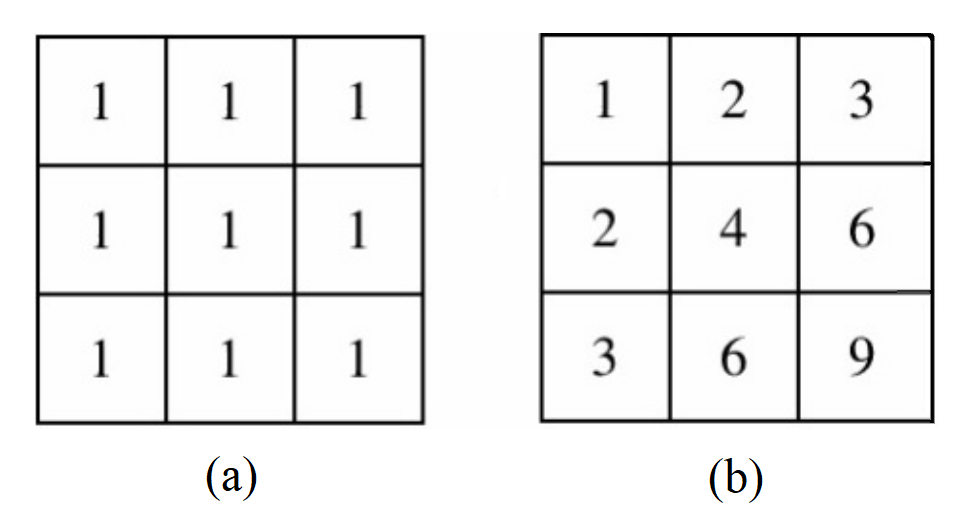
\includegraphics[width=0.5\textwidth]{Figures/integralImage.png}
	\caption{Výpočet integrálneho obrazu - vstupný obraz (A) , integrálny obraz (B)}
	\label{fig:integralImage}
\end{figure}


\begin{equation}
ii(x,y)=\sum_{x^{\prime}\leq x,y^{\prime}\leq y}i(x^{\prime},y^{\prime}),
\label{eq:integral}
\end{equation}


 Metóda funguje na porovnavaní celých blokov pixelov. Tieto bloky (častokrát nazývané aj zhluky) môžu mať rôzne tvary, veľkosť a natočenie. Tieto bloky môžu nadobúdať rôzne tvary ale vo všeobecnosti sa používajú 3 hlavné typy príznakov:
\begin{itemize}
  \item \textbf{Dvoj-obdĺžnikové} \textit{(angl. two-rectangle)} - porovnávajú sumu pixlov v obdĺžnikových oblastiach, ktoré sa nachádzajú vedľa seba, vodorovne, alebo zvislo.
  \item \textbf{Troj-obdĺžnikové} \textit{(angl. three-rectangle)} - porovnávajú sumu obdĺžnikových oblastí, ktoré sa nachádzajú po oboch stranách aktuálnej oblasti a sumu aktuálnej oblasti.
  \item \textbf{Štvor-obdĺžnikové} \textit{(angl. four-rectangle)} - počítajú rozdiel medzi dvoma aktuálnymi obdĺžnikovými oblasťami, ktoré sa dotýkajú svojimi rohmi, a obdĺžnikovými oblasťami medzi nimi.
  
 \end{itemize}
   \begin{figure}[H]
	\centering
	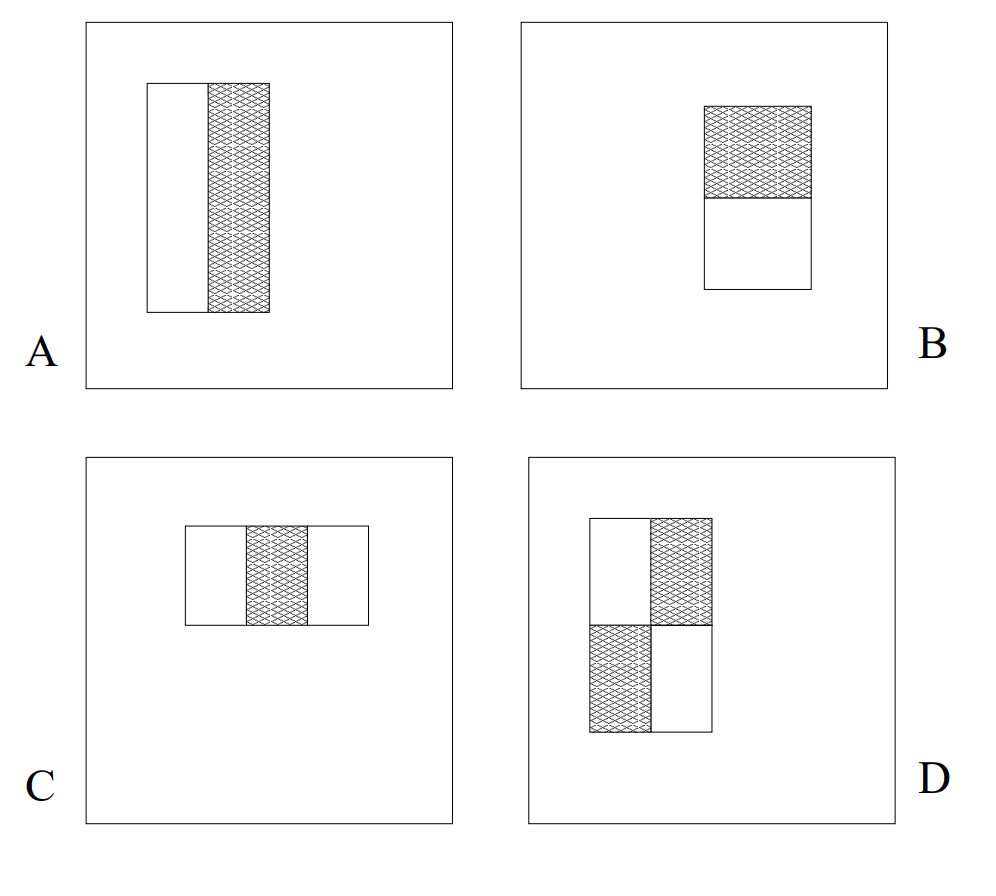
\includegraphics[width=0.6\textwidth]{Figures/haar1.png}
	\caption{Haar - dvoj-obdĺžnikové príznaky (A, B), troj-obdĺžnikové príznaky (C) a štvor-obdĺžnikové príznaky(D)\cite{viola2001robust}}
	\label{fig:Haar1}
\end{figure}
  Znázornenie jednotlivých typov príznakov môžeme vidieť na obrázku \ref{fig:Haar1}. Jednotlivé príznaky môžu byť použité dostatočne efektívne. Efektivita klesá pri použití príznaku na celý obraz. Vhodným riešením je preto skombinovať viacero príznakov. Na výber  správnych efektívnych príznakov sa používajú špeciálne algoritmy. Jedným z najpoužívanejších algoritmov  pre zvýšenie efektivity výberu príznakov je AdaBoost\cite{freund1995desicion}, ktorý vytvoril profesor Yoav Freund. Jedná se o klasifikačný algoritmus, ktorý je schopný vytvoriť dostatočne silný klasifikátor z kombinácii viacerých slabších klasifikátorov.  Metódou Haar je možné detekovať rôzne triedy objektov.  Jedným z najčastejších a jednoducho detekovatelných  typov objektov je napríklad tvár.


\begin{figure}[H]
	\centering
	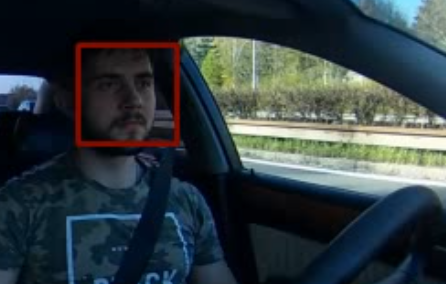
\includegraphics[width=0.6\textwidth]{Figures/haar2.png}
	\caption{Haar - detekcia tváre v slabých svetelných podmienkach}
	\label{fig:Haar2}
\end{figure}



\subsection{HOG}
\label{HOG}
S nápadom  vylepšiť detekciu objektov použitím príznakov prišli v roku 2005 Navneed Dalal a Bill Triggs \cite{dalal2005}, kde postupne vyskúšali niekoľko typov deskriptorov.  V práci taktiež podrobne rozobrali  možnosti a spôsoby ako správne určiť parametre ich detekčnej metódy pre správne fungovanie detekcie jednotlivých tried. Hlavnou myšlienkou ich metódy je, že objekt môže byť charakterizovaný  viacerými spôsobmi. Táto metóda je rozdelená do niekoľkých samostatných krokov (Obr. \ref{fig:HOG1}):
\begin{itemize}
  \item \textbf{Úprava obrazu} - v tomto kroku je potrebné  v obraze upraviť kontrast a jas , ktoré by mohli spôsobovať  problémy v nasledujúcich krokoch. Okrem tejto úpravy  je možné  obraz urpaviť napríklad gamma filtrom.
  \item \textbf{Výpočet gradientov} - veľkosť gradientov sa počíta na základe vstupného obrazu a masky. Masky, ktoré sa používaju v tomto kroku sú \textit{[-1, 0, 1]} alebo \textit{[-1, 0, 1] \textsuperscript{T}}. Gradienty je nutné vypočítať v obidvoch osách, čím získame \textit{I\textsubscript{x}} a \textit{I\textsubscript{y}}. Po získaní gradientov je potrebné vypočítať veľkosť gradientov \textit{m(x,y)} a ich smer \textit{$\theta(x, y)$}:
  
\begin{equation}
m(x,y)= \sqrt{I_{x}^{2} + I_{y}^{2}}
\label{eq:Výpočet veľkosti gradientu}
\end{equation}

  \begin{equation}
\theta(x, y) = \left(\frac{I_{y}}{I_{x}}\right)
\label{eq:Výpočet smeru gradientu}
\end{equation}
  \item \textbf{Normalizácia} -  Pre správne fungovanie je potrebné obraz normalizovať, aby sa minimalizovali rozdiely medzi jednotlivými bunkami. Tento krok spočíva v skladaní viacerých buniek, čím následne vznikajú bloky. 
   \item \textbf{Deskriptor} -  Je vytvorený zo vstupného obrazu do jednotlivých blokov. Jednotlivé bloky sa posúvajú a prekrývajú o daný počet pixelov. Výsledok desktiproru je odovzdaný  klasifikátoru, ktorý následne určuje do akej triedy objekt patrí. Jeden z často používaných klasifikátorov je Support vector machine (SVM), ktorý napríklad používali autori práce na efektívnu detekciu chodcov.\cite{pang2011efficient}
 \end{itemize}


\begin{figure}[H]
	\centering
	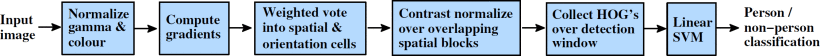
\includegraphics[width=1\textwidth]{Figures/hog.png}
	\caption{HOG - séria krokov \cite{dalal2005}}
	\label{fig:HOG1}
\end{figure}

Výstupom tejto metódy je pole histogramov pre jednotlivé bloky. Histogram predstavuje grafické rozloženie intenzity jasu vstupného obrazu. Pri niektorých špecifických obrazoch je potrebné histogram vyrovnať. Tento krok je potrebný najmä pri obrazoch, ktoré su príliš tmavé alebo príliš svetlé. Pomocou vyrovnania \textit{(angl. equalization)} histogramu  dokážeme zvýšiť kontrast obrazu. Jednotlivé kroky znázornené na vstupnom obraze chodca môžeme vidieť na obrázku \ref{fig:HOG2}\par


\begin{figure}[H]
	\centering
	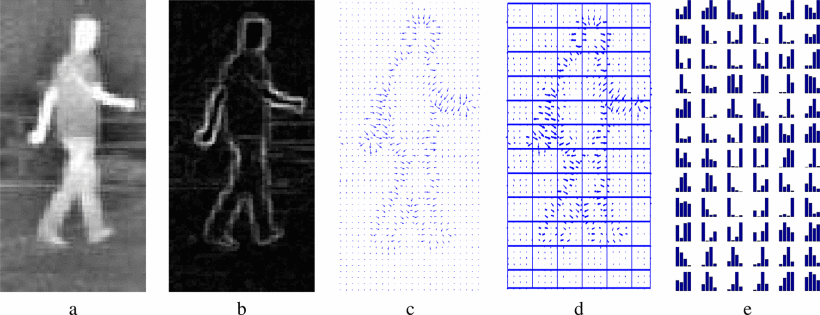
\includegraphics[width=1\textwidth]{Figures/hog3.png}
	\caption{HOG - vstupný obraz (a), normalizácia gradientu (b), orientácia gradientu (c), rozdelenie do buniek (d) vypočítané histogramy (e). \cite{bertozzi2007pedestrian}}
	\label{fig:HOG2}
\end{figure}


\newpage
\subsection{OpenPose}
OpenPose\cite{cao2018openpose} je framework, ktorý bol prvýkrat uvedený verejnosti už v roku 2016. Detekcia ľudského postoja predstavuje hlavný problém s lokalizáciou častí ľudského tela, ako sú ramená, lakte a členky zo vstupného obrázka alebo videa. Vo väčšine dnešných aplikácií detekcie postaáv v reálnom svete sa vyžaduje vysoký stupeň presnosti, ako aj spracovanie v reálnom čase.
OpenPose, ktorý bol vyvinutý výskumníkmi na univerzite Carnegie Mellon University, možno považovať za najmodernejší prístup pri detekcii ľudských v reálnom čase. Jedná sa o open-source projekt, ktorého zdrojové kôdy sú dostupné na oficiálnej Github stránke \cite{githubOpenpose}.

\begin{figure}[H]
	\centering
	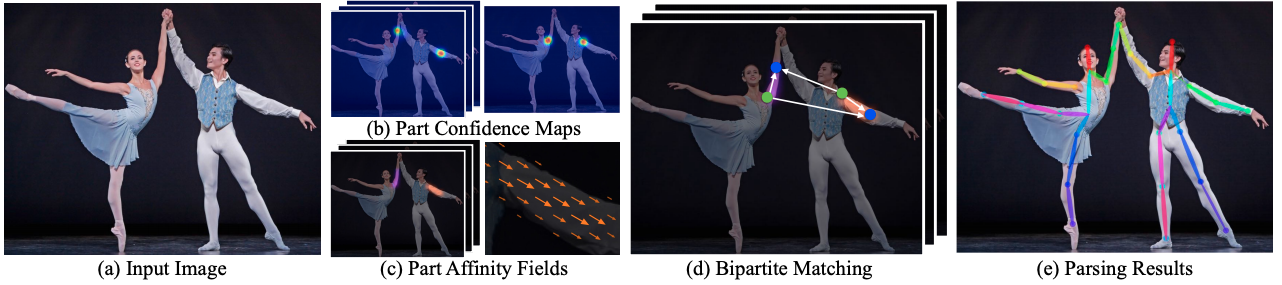
\includegraphics[width=1\textwidth]{Figures/openposePipeline.png}
	\caption{OpenPose - odhad viacerých ôsob v reálnom čase pomocou polí afinity filtra.\cite{cao2018openpose}}
	\label{fig:openposeOverall}
\end{figure}

 Samotný framework je veľmi detailne vysvetlený a dobre zdokumentovaný. OpenPose bol pôvodne napísaný v C++ a Caffe\cite{jia2014caffe}. Postupom času však  autori vytvorili aj  nadstavbu pre jazyk Python, s ktorým sa rozšírili možnosti jeho využitia medzi ostratnými programátormi. Základná myšlienka detekcie pomocou OpenPose sa skladá z viacerých krokov:

\begin{itemize}
\item \textbf{Spracovanie vstupného obrazu} - vstupný obrázok (Obr. \ref{fig:openposeOverall}a) privádza ako vstup do „dvojvetvového viacstupňového“ CNN. Dve vetvy znamenajú, že CNN produkuje dva rôzne výstupy z jedného vstupného obrazu. Viacstupňové jednoducho znamená, že sieť je v každej fáze naskladaná jedna na druhú. (Tento krok je analogický jednoduchému zväčšeniu hĺbky neurónovej siete s cieľom zachytiť podstatnejšie výstupy smerom k posledným stupňom.)

\item \textbf{Spracovanie v dvoch vetvách} - prvá vetva predpovedá mapy dôveryhodnosti (Obr. \ref{fig:openposeOverall}b) rôznych častí tela, ako je pravé oko, ľavé oko, pravé lakte a podobne. Druhá vetva zobrazená modrou farbou predpovedá afinitné polia (Obr. \ref{fig:openposeOverall}c), čo predstavuje stupeň asociácie medzi rôznymi časťami tela.

\item \textbf{Viacfázové spracovanie} - v prvej fáze sieť vytvorí počiatočnú sadu detekčných máp spoľahlivosti \textit{S} a množinu polí afinity častí \textit{L}. Potom v každej nasledujúcej fáze predpovede z obidvoch vetiev v predchádzajúcej fáze, spolu s pôvodnými obrazovými znakmi \textit{F}, sú zreťazené a použité na vytvorenie podrobnejších predpovedí. Pri implementácii OpenPose sa posledná fáza \textit{t} zvolí ako  číslo 6.
\end{itemize}

\subsubsection{Mapa spoľahlivosti}
1. vetva v neurónová sieti OpenPose vytvára sadu máp spoľahlivosti \textit{S} (rovnica \ref{eq:confidencemap}). V podstate sa jedná o tabuľku, v ktorej je každej časti tela z datasetu priradená miera spoľahlivosti v rozsahu 0 až 1. 

\begin{eqnarray}
& S = (S_{1}, S_{2}, S_{3} ... S_{j}) \label{eq:confidencemap}\\
& S\in\mathbb{R}^{w \times  h},\nonumber\\
& j\in \left \{1,\: J  \right \}, kde\: J\: je\: počet\: všetkých\: častí\: tela\nonumber
\end{eqnarray}
Počet častí tela závisí od množiny datasetov, s ktorými je program OpenPose trénovaný. Pokiaľ ide napríklad o súbor datasetu COCO\cite{lin2014microsoft}, \textit{J = 19}, pretože existuje 18 rôznych kľúčových bodov tela + 1 pozadie. Obrázok \ref{fig:cocoDataset} zobrazuje rôzne časti tela s prideleným ID pre súbor údajov COCO. Pre model trénovaný s dátovým súborom COCO bude sada \textit{S} obsahovať prvky \textit{S1, S2, S3,…, S19}. V tomto príklade predpokladáme, že prvok \textit{S1} zodpovedá mape spoľahlivosti pre kľúčový bod s číslom 0 ktorý zodpovedá nosu (Obr. \ref{fig:cocoDataset}).\par Pre ľahšiu predstavu predpokladáme, že celý obraz má šírku a výšku 5px, čo vedie k vytvoreniu  mapy spoľahlivosti o veľkosti 5 X 5. Vo vstupnom obrázku sa nachádza iba jedna tvár. Preto pre mapu spoľahlivosti \textit{S1} (zodpovedajúca za detekciu nosa) vidíme hodnoty s vysokou spoľahlivosťou iba v oblasti, kde sa nos nachádza.\bigskip

\begin{figure}[H]
	\centering
	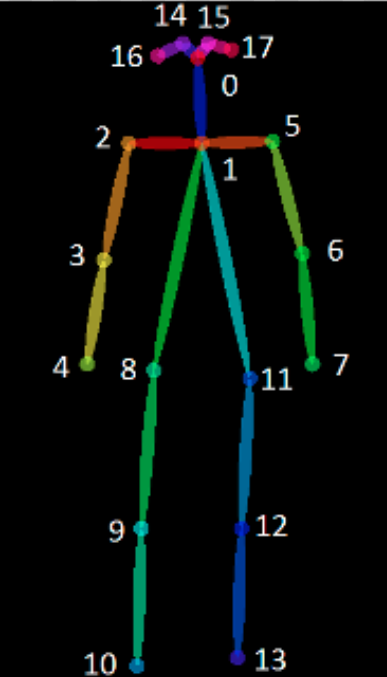
\includegraphics[width=0.3\textwidth]{Figures/cocoDataset.png}
	\caption{COCO - označenie častí tela v COCO datasete.\cite{cocoDataset}}
	\label{fig:cocoDataset}
\end{figure}


\subsubsection{Part afinity fields (PAF)}
Druhá vetva neurónovej siete vytvára množinu čiastkových afinitných polí \textit{L} (rovnica \ref{eq:pafmap}).

\begin{eqnarray}
& L = (L_{1}, L_{2}, L_{3} ... L_{c}) \label{eq:pafmap}\\
& L\in\mathbb{R}^{w \times  h \times 2},\nonumber\\
& c\in \left \{1,\: C  \right \}, kde\: C\: je\: počet\: všetkých\: končatín\nonumber
\end{eqnarray}

Celkový počet končatín a párov, závisí od datasetu, s ktorým je OpenPose trénovaný. Kvôli prehľadnosti sa uvádzajú dvojice častí tela ako končatiny, napriek tomu, že niektoré páry častí tela nie sú v skutočnosti končatinami (Napríklad oko-nos, ucho-oko atď). Pre dataset COCO je počet párov končatín, \textit{C = 19}. Môžeme si predstaviť, že každý prvok v množine \textit{L} je mapa veľkosti \textit{$w\times h$}, kde každá bunka obsahuje 2D vektor predstavujúci smer párových prvkov. Napríklad na obrázku \ref{fig:cocoDataset} môžeme vidieť, že pár častí tela pozostáva z pravého ramena k pravému laktu. Schéma potom ukazuje smerový vektor, ktorý ukazuje z pravého ramena na pravý lakeť. Celý zoznam párov končatín môžeme vidieť vo výpise \ref{src:coco_pairs}.\bigskip

\begin{lstlisting}[language=Python,label=src:coco_pairs,caption={Množina párov končatín v datasete COCO}]
COCO_PAIRS = [(1, 2), (1, 5), (2, 3), (3, 4), (5, 6), (6, 7), (1, 8), (8, 9), (9, 10), (1, 11), (11, 12), (12, 13), (1, 0), (0, 14), (14, 16), (0, 15), (15, 17), (2, 16), (5, 17)]
\end{lstlisting}

\bigskip
Okrem Datasetu COCO Dokáže OpenPose pracovať aj s mnohými ďalšími datasetmi. OpenPose bol skúšaný a trénovaný napríklad s datasetmi MPI, BODY\_25 alebo BODY\_25b. Datasety sa líšia vo veľkosti, rýchlosti, ale napríklad  aj v presnosti samotnej detekcie. Jednotlivé datasety majú medzi sebou nasledujúce rozdiely:


\begin{itemize}
\item \textbf{COCO} - je starší dataset, na ktorom bol OpenPose pôvodne vyvíjaný. Postupne sa však nahradzuje novými a modernejšími datasetmi. Jeho výhodou je, že vyžaduje menej pamäte na GPU (schopnosť pracovať s 2 GB GPU a predvoleným nastavením) a pri režíme CPU pracuje rýchlejšie oproti novšiemu BODY\_25.

\item \textbf{BODY\_25} - jedná sa o novší dataset, ktorý je rýchlejší, presnejší a obsahuje ďalšie trénovacie dáta k častiam tela, ktoré nie sú obsiahnuté v COCO datasete (Napr. chodidlá). Jeho nevýhodou sú hlavne vysoké hardwarové nároky.

\item \textbf{MPI} - je určený pre ľudí, ktorí požadujú štruktúru datasetu MPI. Je tiež pomalší oproti BODY\_25 a oveľa menej presný
\end{itemize}




\newpage
\subsection{TensorFlow}
tensorflow


\newpage
\subsection{Ostatné metódy}
WrnchAI je pomerne novy framwework, nieje  opensource

\newpage
\section{Detekcia vodiča vo vozidle}
\label{sec:Pose detection}
Detekcia objektov v uzavretom priestore (v našom prípade vo vozidle) sa od bežnej detekcie v základných princípoch nelíši. Obmedzenia nastávaju najmä nevhodnou pozíciou alebo natočením kamery. Ak je kamera nesprávne umiestnená, alebo má nedostatočný uhol záberu, nemusí byť zdetekovaný celý snímaný objekt, čo môže viesť k chybe pri jeho detekcii. Autori v práci \cite{smith2003determining}, kde sa zameriavali na oblasť tváre vodiča použili kameru umiestnenú v oblasti stredu palubnej dosky. Tým dosiahli takmer priame natočenie kamery na vodiča , bez toho, aby ho táto kamera výraznejšie obmedzovala vo výhľade. Keďže táto práca bola zameraná hlavne na detekciu  očí a úst, nebolo potrebné  používať kameru s vysokým uhlom záberu. Mnoho podobných riešení zameraných na snímanie aktivity vodiča sa snaží zaviesť mnoho výrobcov automobilov. Príkladom môže byť vyrobca  automobilov značky BMW, ktorý v príplatkovej výbave ponúka kameru na snímanie správania vodiča. Táto kamera dokáže reagovať napríklad na únavu alebo zatvorenie očí vodiča. Tento systém dokáže dokonca reagovať aj na to, že vodič má otočenú hlavu a nesleduje premávku. V každom takomto prípade je vodič upozornenený zvukovým znamením. Kamera je umiestnená na mieste, odkiaľ je na tvár vodiča priamy výhľad (Obr. \ref{fig:bmwAssistent}). Okrem jej vhodného umiestnenia je navyše vybavená aj IR LED diódami, vďaka ktorým kamera funguje aj za znížených svetelných podimenok a v noci, kedy sa vyskytuje najväčší počet mikrospánkov u vodičov vozidiel.

\begin{figure}[H]
	\centering
	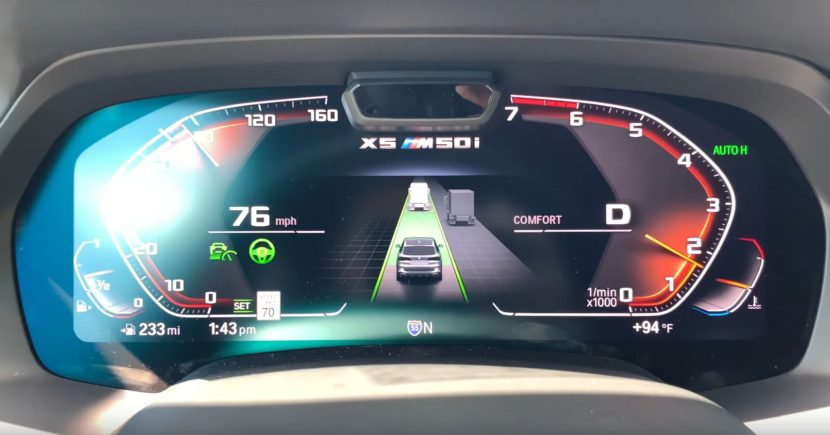
\includegraphics[width=0.6\textwidth]{Figures/bmw.jpg}
	\caption{BMW driving assistent - umiestnenie kamery na snímanie vodiča.\cite{bmw2019assistent}}
	\label{fig:bmwAssistent}
\end{figure}

 Táto diplomová práca je však zameraná aj na detekciu celého tela vodiča a nielen jeho tváre. 







\newpage
\section{Využitie sférických kamier na detekciu obrazu}
\label{sec:Spherical cameras}

\newpage
\subsection{Použitie v analýze videa}
- problem s rozlišenim , skreslenim , formatom atd.. 
- 


\subsection{Technické parametre}
Go PRO:

THETA:

Senzor	FishEye CMOS 2x12MPix
Maximálne rozlíšenie (Video)	4K  30fps
Maximálne rozlíšenie (Fotografia)	14.5MP (5376x2688px)
Svetelnosť	f2.0
Vnútorná pamäť	19GB

\newpage
\section{Program}
\label{sec:Program}
- Popis programu\\
- jazyk Python\\
- pouzite kniznice\\


\newpage
\subsection{Požiadavky a návrh programu}
- poziadavky \\
- Architekruta programu , schemy


\newpage
\subsection{Detekcia vodiča}
- umiestnenie kamery, detekcia vodiča\\
 - vyber TF vs OpenPose



\newpage
\subsubsection{Neurónová sieť}
-NN klasifikator\\
- trenovanie \\
- testovanie



\newpage
\subsection{Orientácia hlavy}
- Haar  priznaky ,\\
- prevod 2D na 3D \\
- smerova priamka

\newpage
\subsection{Výstup programu}
obrazky\\
tabulky

\newpage
\subsection{Porovnanie výsledkov}
porovnanie


\newpage
\subsection{Využitie zozbieraných dát}
pouzitie v buducnosti


\newpage
\subsection{Používateľská príručka}
python program.py --use-openPose=true


\newpage
\section{Možnosti vylepšenia detekcie}
\label{sec:Možnosti vylepšenia detekcie}
Zhrnutie vysledkov


\newpage
\section{Záver}
\label{sec:Zaver}
Zhrnutie vysledkov







\bibliography{literatura}














\end{document}
